%%%% lwa-submit.tex
\typeout{LWA Submission Instructions for Authors}

% These are the instructions for authors for LWA.
\documentclass[a4paper]{article}
%\documentclass[pdftex,bibtotocnumbered,idxtotoc,11pt]{scrartcl}

% The file lwa.sty is the style file for LWA.
\usepackage{lwa}

% Use the postscript times font!
\usepackage{times}
\usepackage{latexsym}

%\documentclass[pdftex,bibtotocnumbered,idxtotoc,11pt]{scrartcl}
\usepackage{amsmath,amsfonts}
\usepackage{xcolor,graphicx,fancybox,wrapfig}
\usepackage{url,acronyms,myref,locutor}
\usepackage{wasysym}
\usepackage{listings}
\usepackage{lstomdoc}
\usepackage{xmlindex}
\usepackage{tikz}
\usepackage[hide]{ed}
\usepackage[margin={2.5cm,2.5cm,1.5cm,1.5cm}]{geometry}


% Load this last!
\usepackage{hyperref}
%%

\lstset{float=htb,columns=flexible,frame=lines,language=[omdoc]XML,basicstyle=\scriptsize,
        indexstyle=\indextt,indexstyle=[1]\indexelement,indexstyle=[2]\indexattribute,
        showstringspaces=false}

\newcommand{\PC}{\mathcal{PC}}
\renewcommand{\mod}{\operatorname{mod}}
\def\javascript{{\sc{JavaScript}}}
\def\llquote#1{\ensuremath{\langle\kern-.25em\langle\hbox{\sl{#1}}\rangle\kern-.25em\rangle}}
\def\pres#1#2{\overline{#1}^{#2}}  
\def\lden{[\kern-.15em[}\def\rden{]\kern-.15em]}
\def\defemph#1{{\bf{#1}}}
\def\imarg#1#2{\fbox{\ensuremath{\left.#1\right|_{#2}}}}
\def\fimarg#1#2#3{\fbox{\ensuremath{\left.#1\right|_{#2}^{#3}}}}
\def\recu#1{#1}%should be changed to notation for <recurse precedence="#1"/>, maybe a circle around p

\def\name#1{{{\small{\sc{#1}}}}}


% \makeatletter
% \renewcommand\paragraph{\@startsection{paragraph}{4}{\z@}%
% {1.25ex \@plus1ex \@minus.2ex}%
% {-1em}%
% {\setlength{\parfillskip}{\z@ \@plus 1fil}%
% \raggedsection\normalfont\sectfont\nobreak
% \size@paragraph\nobreak}}
% \makeatother

\title{Presenting Mathematical Content With Flexible Elisions}
\author{Michael Kohlhase, Christoph Lange, Florian Rabe\\ 
  Computer Science, Jacobs University Bremen\\
  D-28759 Bremen, Germany \\ 
  {\small\url{m.kohlhase/ch.lange/f.rabe@jacobs-university.de}}}
\date{}

\begin{document}
\maketitle

\begin{abstract}%\vspace*{-.7cm}
  Mathematicians frequently elide brackets or symbols in formulae to concentrate on
  essential facts and to avoid distracting experienced mathematicians with notation that
  can easily be deduced from context. In this paper we propose a extension of the notation
  specification infrastructure in {\omdoc} by functionality for flexible elisions.
\end{abstract}

\section{Introduction}\label{sec:intro} 

Over the last three millennia, mathematics has developed a complicated two-dimensional
format for communicating formulae (see e.\,g.~\cite{Cajori:ahmn93,Wolfram:mnpf00} for
details). Changes in notation have been influential in shaping the way we calculate and
think about mathematical concepts, and understanding mathematical notations is an
essential part of any mathematics education.

Content Markup formats for mathematical formulae such as
{\openmath}~\cite{BusCapCar:2oms04} and {\mathml}~\cite{CarIon:MathML03} concentrate on
their functional structure, thus allowing mathematical software systems to exchange
mathematical objects. For communication with humans, these formats rely on a
``presentation process'' (usually based on XSLT style sheets) that transforms the content
objects into the usual two-dimensional form used in mathematical books and articles.

After a conceptual analysis of the presentation process and a survey of recent approaches
to specify the notations of mathematical symbols and how to use these specifications to
transform content-oriented mathematical documents to a presentation-oriented format like
PDF or HTML, we introduce a revised specification of the presentation module of the
{\omdoc}~\cite{Kohlhase:omdoc1.2} language that is enabled for elisions.  We conclude by
proposing how information about elisions that a presentation algorithm performed can be
included in the presentation markup and used by a client application.

\subsection{Presentation as Composition and Elision}

Many such presentation processes have been proposed, and all have their strengths and
weaknesses. In this paper, we conceptualize the presentation of mathematical formulae as
consisting of two components: the two-dimensional {\defemph{composition}} of visual
sub-presentations to larger ones and the {\defemph{elision}} of formula parts that can be
deduced from context.

Most current presentation processes concentrate on the relatively well-understood
composition aspect and implement only rather simple bracket elision algorithms. But the
visual renderings of formulae in mathematical practice are not simple direct compositions
of the concepts involved: mathematicians gloss over parts of the formulae, e.\,g.\ leaving
out arguments, iff they are non-essential, conventionalized or can be deduced from the
context. Indeed this is part of what makes mathematics so hard to read for beginners, but
also what makes mathematical language so efficient for the initiates. A common example is
the use of $\log(x)$ or even $\log x$ for $\log_{10}(x)$ or similarly $\lden t\rden$ for
$\lden t\rden_{\cal M}^\phi$, if there is only one model $\cal M$ in the context and
$\phi$ is the most salient variable assignment. Another example are the bracket elision
rules in arithmetical expressions: $ax+y$ is actually $(ax)+y$, since multiplication
``binds stronger'' than addition. Note that we would not consider the ``invisible times''
operation as another elision, but as an alternative presentation. Finally, there are
extreme examples of elision or substitution like Church's dot notation, where a dot stands
for a left bracket, whose mate is as far to the right as consistent with the remaining
(un-elided) brackets. For instance $(a\cdot.\,b+c)-d$ stands for $(a\cdot(b+c))-d$, and
$\forall x,y.\phi\wedge\psi$ stands for $\forall x,y (\phi\wedge\psi)$.

Now that we have convinced ourselves that the elision is an important component of
generating high-quality presentations, let us reconsider the presentation process itself
to see how composition and elision interact.

We will start from the observation that in content markup formalisms for mathematics
formulae are represented as ``formula trees''. Concretely, we will concentrate on
{\openmath} objects, the conceptual data model of {\openmath} representations, since it is
sufficiently general, and work is currently under way to re-engineer content {\mathml}
representations based on this model. Furthermore, we observe that the target of the
presentation process is also a tree expression: a layout tree made of layout primitives
and glyphs, e.\,g.\ a presentation {\mathml} expression. If we make examples with
{\TeX/\LaTeX}, it is only since it is universally understood; here, the layout tree is the
parse tree implicit in the linear {\TeX/\LaTeX} string. This notwithstanding, we finally
observe that even though formula presentations are two-dimensional in principle, large
parts are more or less linear, and therefore mathematical notation relies on brackets to
allow the reader to reconstruct the content structure from the presentation.

\subsection{Characteristics of Mathematical Symbols}\label{sec:characteristics}

In a nutshell, {\openmath} objects are trees built up from {\defemph{variables}} and
{\defemph{symbols}} at the leaves and {\defemph{applications}} and {\defemph{binders}} as internal
nodes. 

\begin{wrapfigure}{r}{3cm}\vspace*{-.5em}
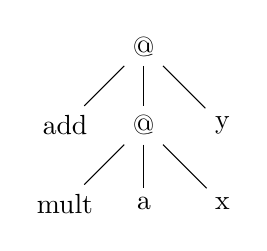
\begin{tikzpicture} 
\node (top) at (1,2) {@};
\node (plus) at (0,1) {add};
\node (mid) at (1,1) {@};
\node (y) at (2,1) {y};
\node (mult) at (0,0) {mult};
\node (a) at (1,0) {a};
\node (x) at (2,0) {x};
\draw(top) -- (plus);
\draw(top) -- (mid);
\draw(top) -- (y);
\draw(mid) -- (mult);
\draw(mid) -- (a);
\draw(mid) -- (x);
\end{tikzpicture}\vspace*{-.5em}
\end{wrapfigure}
For our purposes, symbols and applications are the most important concepts,
therefore let us fortify our intuition with the example on the right: the sum $ax+y$ above
would be represented by a tree with an application at the root, whose first child is the
symbol\footnote{Note that a symbol is not a glyph --- these are often confused, the symbol
  here stands for the mathematical concept of a sum, not the glyph $+$.} for addition, the
third child is the variable with the name $y$, and the second child is another application
whose children are the symbol for multiplication and the variables with names $a$ and $x$.

As part of the functional notation of mathematics popularized by Leibniz and Newton for
algebra, the visual appearance of a subformula was largely determined by its head
operator, which nowadays carries much of the notational conventions, which are usually
phrased in terms of the following notational characteristics of a symbol:

\begin{description}
\item[fixity (for operators):] Is the operator displayed as a prefix (like a function
  symbol), as a postfix (like the factorial symbol $!$) or as an infix (like most
  arithmetic operators)?  Operators of higher arity can also have a ``mixfix'' style;
  consider the 4-ary typing judgment operator $\Gamma\vdash_\Sigma t\colon\alpha$, which
  states that a term $t$ has type $\alpha$ in a variable context $\Gamma$ and a signature
  $\Sigma$.
\item[left and right brackets:] If an operation is bracketed, are round, square, curly,
  angle, or other brackets used? In fact brackets in mathematical vernacular are mostly
  round brackets; technical notations sometimes use others, e.g. {\mathematica} uses
  square ones throughout. Note that not all parts of a presentation that look like
  brackets are indeed. For instance in a half-open interval as $]a;b]$, is actually mixfix
  operator where the bracket-like glyphs ``$]$'' look and conventionally stretch like
  brackets, but do not match and cannot be elided like brackets. They are easy to mistake
  for brackets, since they (as all fully inhabited mixfix presentations) make brackets for
  the arguments unnecessary. We would consider it a semantic anomaly to present an
  ``interval'' operator as an infix ``;'' with obligatory left and right brackets ``$]$''
  and ``$]$''.
\item[precedence (for operators):] If an operation $O$ with a high precedence occurs as an
  argument of an operator with a lower precedence, the brackets around $O$ can be
  elided.
\item[associativity (for infix operators):] To elide brackets for $n$-ary operators
  ($n>2$), it must be known whether they are associative (i.\,e.\ $(a\circ b)\circ c =
  a\circ(b\circ c) =: a\circ b\circ c$) or obey ``left-associative'' or
  ``right-associative'' elision conventions (e.g.
  $\alpha\to\beta\to\gamma:=\alpha\to(\beta\to\gamma)$ for right-associative function
  types).
\end{description}
The first two characteristics specify the composition of the visual representations,
whereas the latter two are concerned with bracket elision. Furthermore, the {\bf{role}} of
a symbol in the formula context needs to be taken into account: Is it a simple
{\emph{constant}} like $\mathbb{R}$, a {\emph{function}} that is applied to arguments, or
a {\emph{binder}} that binds variables like $\forall x.p(x)$. This is most pronounced for
functions that can occur either applied to arguments or as the concept alone.
Presentations differ for these occasions, e.g. for the absolute value function, we write
something like $\bigl|\cdot\bigr|$ with a ``dummy argument'' $\cdot$ when it is not in an
applied context.

\subsection{Notation Definitions}\label{sec:notdef}

Mathematical formulae given in the XML-based structural formats {\openmath} and Content
{\mathml} are commonly presented by implementing one XSLT template~\cite{W3C:xslt2} per
symbol, which specifies how to transform this symbol to the output format---another XML
format like Presentation {\mathml}, or a non-XML format like {\TeX}, for example.
Appropriate templates for the arguments are usually applied recursively.

The following listing shows a straightforward way to transform the exponentiation operator
from {\openmath} to {\TeX}:
 
\begin{lstlisting}[language=XSLT,caption=An XSLT presentation template,label=lst:template]
<xsl:template match="om:OMA[om:OMS[@cd='arith1'
 and @name='power']]">
  <xsl:apply-templates select="*[2]"/> <!-- first argument -->
  <xsl:text>^{</xsl:text>
  <xsl:apply-templates select="*[3]"/> <!-- second argument -->
  <xsl:text>}</xsl:text>
</xsl:template>
\end{lstlisting}

To save authors from the tedious and error-prone task of writing similar templates for
every symbol and notation variant, different facilitations have been invented. The
probably earliest examples were the presentation architecture in
{\omdocv{1.0}}~\cite{Kohlhase:otormd00} and Naylor's \& Watt's {\openmath}
conversion~\cite{Naylor:conversion}. Both supply XML-based {\defemph{notation
    definitions}} that can be transformed into a suitable XSLT conversion style sheet by a
meta-stylesheet.

In {\omdoc}, a template like the one above would be generated from a
{\element{presentation}} element of the form
\begin{lstlisting}[mathescape]
<presentation for="power" theory="arith1" role="application" class="1">
  <style format="TeX">
    <recurse select="*[2]"/><text>^{</text>
    <recurse select="*[3]"/><text>}</text>
  </style>
  $\ldots$
<presentation>
\end{lstlisting}
where the {\attribute[ns-elt=xsl]{match}{template}} attribute is generated from the
attributes on the {\element{presentation}} element and the contents from the ones on the
{\element{use}} element. In contrast to this, where notations definitions are thought as
directed rules from content to presentation, Naylor's \& Watt's framework views them as
equivalences between representations. For the example above we would have
\begin{lstlisting}[mathescape,language=XML,morekeywords={Notation,version,semantic-template},
caption=A Template-Based Notation Definition,label=lst:template-based]
<Notation>
  <version style="1">
    <tex>\arg{a1}{n}^{\arg{a2}{m}}</tex>
    $\ldots$
  </version>
  <semantic-template>
    <OMA><OMS cd="power" name="arith1"/>
      <OMV name="n" id="a1/>
      <OMV name="n" id="a2/>
    </OMA>
  </semantic-template>
</Notation>
\end{lstlisting}
We will call the first approach to notation specification {\defemph{symbol-based}}, as the
notation is tied to a concrete symbol, and the second one {\defemph{template-based}}. Note
that the template-based approach is in principle more directly invertible (e.g. for
parsing), and more expressive (it would e.g. allow to present $log(e,x)$ as $\ln(x)$ and
$log(b,x)$ as $\log_b(x)$). But this has not been realized in practice, since the
presentation of mathematical formulae {\emph{is indeed}} tied to symbols, so all templates
are indeed one-level like the one in the example above. On this fragment, both approaches
are equivalent. Note furthermore that many of the notational characteristics of a symbol
mentioned in section~\ref{sec:characteristics} actually do not belong to the symbol but to
its presentation. For example, the division operator, presented as $\cdot/\cdot$, has a
higher precedence than $\frac{\;\cdot\;}{\;\cdot\;}$---consider $1/(a+b)$ vs.\
$\frac{1}{a+b}$.

In {\omdocv{1.2}}~\cite{Kohlhase:omdoc1.2}, all of these characteristics can be specified
as attributes to one out of potentially multiple {\element{presentation}} elements that
refer to a {\element{symbol}}. For some aspects like mix-fixity, this declarative syntax
is not yet expressive enough; in this case, embedded XSLT templates must be used, losing
declarativity. In this paper, we rethink the notation definition system and propose a
declarative system extending ideas from the notation definition system in the {\isabelle}
theorem proving environment~\cite{Paulson:Isabelle05}.

\section{A Mixfix Presentation Model for Flexary Terms}\label{sec:flexary}
The {\isabelle} presentation process allows to model all of the symbol characteristics
discussed in section~\ref{sec:characteristics} by a single notation definition: the
{\defemph{mixfix declaration}}. For an $n$-ary symbol, $f$ is a declaration of the form
$w_0\imarg{p_1}{\pi_1}w_1\imarg{p_2}{\pi_2}\ldots\imarg{p_n}{\pi_n}w_n:p$, where the $w_i$
are strings in the output language and $p$ is the {\defemph{output precedence}} of $f$. We
call the boxes {\defemph{argument specifications}}, the $p_i$ are {\defemph{input
    precedences}}. In accordance with Prolog, which, in contrast to {\isabelle},
predefines precedences for many common mathematical operators, and staying compatible with
previous {\omdoc} standards, we assign low precedence values to strongly binding operators
and high precedence values to weakly binding operators.

In the presentation process, a term $t$ is presented as a string
$\pres{t}{q}$, given an initial precedence $q$, according to the following definition:
\[\pres{f(t_1,\ldots,t_n)}{q}=w_0\pres{t_{\pi_1}}{p_1}w_1\ldots w_{n-1}\pres{t_{\pi_n}}{p_n}w_n\]
Note that the $w_i$ contain meta-tokens for brackets (actually pretty-printing blocks that
also handle indentation in {\isabelle}) that will be elided according to the ``current
precedence'' at that point.

A declaration of a right-associative infix operator $\to$ with precedence $p$ can be
modeled by a mixfix declaration $\imarg{p-1}{1}\to\imarg{p}{2}:p$. That means, the first
argument must be an atom or an operator that binds stronger than $\to$, or is bracketed
otherwise, and the second argument must have a maximum output precedence of $p$, which
would present an input of $a\to (b\to c)$ as $a\to b\to c$.

However, the {\isabelle} model is not directly applicable to presentation of {\openmath}
objects, as {\isabelle} crucially depends on the assumption that terms have a fixed arity.
In {\openmath} objects, applications can have flexible arities depending on the operator,
i.\,e.\ application nodes can have different numbers of children, even if they coincide in
the first child (the function). This is used to model a {\defemph{flexary}} addition
function, i.\,e.\ a function that takes any number of arguments, e.\,g.\ $@(add,1,2,3,4)$.
In {\isabelle}, we would have to model addition as a binary, associative operator, and the
term above as $plus(plus(1,2),plus(3,4))$ which would have the same presentation
$1+2+3+4$, but a different structure. Similarly, {\isabelle} only supports unary binding
constructions.

We will now extend the presentation model to the flexary case, and the types of
{\openmath} objects not covered by {\isabelle}, and come back to flexible elision and
abbreviation of non-brackets (we will come back to this in section~\ref{sec:elision}).
  
The first part of the flexary extension is to generalize the idea of an argument vector,
to a list of {\defemph{components}} of an {\openmath} object $O$ as follows (where indices
starts at $0$):
\begin{itemize}
\item for applications and errors: the list of children of $O$, e.\,g.,
  $(f,a_1,\ldots,a_n)$ for the object $@(f,a_1,\ldots,a_n)$,
\item for bindings: the binder, followed by the list of variables, followed by the body,
  e.\,g., $(b,x_1,\ldots,x_n,a)$ for the binding $\beta(b;x_1,\ldots,x_n;a)$,
\item for attributions: a three-element list consisting of the key and the value of the
  first attribution and the original object with the first attribution removed, e.\,g.,
  $(k_1,v_1,\alpha(k_2\mapsto v_2,\ldots,k_n\mapsto v_n;a))$ for $\alpha(k_1\mapsto
  v_1,\ldots,k_n\mapsto v_n;a)$,
\item otherwise: the object itself as a one-element list.
\end{itemize}
As a running example, consider the space of $n$-ary functions. We can model the function
space constructor as a flexary function symbol ${\sf{nfuns}}$ whose last argument is the
codomain and all previous ones the domains. We would like to present an {\openmath} object
$O\colon=@({\sf{nfuns}},A_1,\ldots,A_n,C)$ as $A_1\times \cdots \times A_n\to C$. By the
definition above, the set of components of the object $O$ is the list
${\sf{nfuns}},A_1,\ldots,A_n,C$.

In an obvious generalization of the mixfix notations, we would like to represent the
notation definition for $\sf{nfuns}$ as
$\fimarg{\times:\recu{p-1}}{1}{n-1}\to\imarg{\recu{p}}{n}:p$. In this, we had to
generalize the argument specification for the domains so it can deal with an argument
list. The new {\defemph{argument mapping specification}} represented by the box here
specifies the range of components it covers (the first $n-1$ arguments in our example),
their input precedence\footnote{Note that the input precedences of all members of the
  component range is equal, since they are indistinguishable as list members.}, and
finally, the {\defemph{separator}}, (the $\times$ operator in our example). The
precedences are chosen so that the arrows associate to the right in our example.
  
The general form a of a component mapping specification is $\fimarg{sep:N}be$, where $sep$
is the separator, $N$ is an arbitrary notation that may contain $\recu{p}$ to recurse into
the arguments with input precedence $p$, and $b/e$ are the {\defemph{component sequence
    begin/end indices}}.

Now let $w_0\fimarg{s_1:\recu{p_1}}{b_1}{e_1}w_1\ldots
w_{n-1}\fimarg{s_n:\recu{p_n}}{b_n}{e_n}w_n:p$ be a notation declaration for a function
$f$, then

\[
\begin{array}{l}\pres{@(f,t_1,\ldots,t_m)}{q}=\\
  w_0\pres{t_{b_1}}{p_1}s_1\ldots s_1\pres{t_{e_1}}{p_1}w_1\ldots
        w_{n-1}\pres{t_{b_n}}{p_n}s_n\ldots s_n\pres{t_{e_n}}{p_n}w_n
\end{array}
\]
Note that an {\isabelle}-style argument specification $\imarg{p}\pi$ can be regained as
  $\fimarg{\epsilon:\recu{p}}\pi\pi$, where $\epsilon$ is e.\,g.\  the empty
  string. This legitimizes our example above.

  Note that again, the $w_i$ can contain brackets and other material that can be elided
  taking precedence and other factors into account. We will describe the necessary
  infrastructure at a conceptual level in the next section. 

\section{Flexible Elisions}\label{sec:elision}

There are several situations in which it is desirable to display only some parts of the
presentation:
\begin{itemize}
\item Brackets that are redundant due to operator precedences can be omitted.
\item Arguments that are strictly necessary are omitted to simplify the notation, and the
  reader is trusted to fill them in from the context.
\item Arguments are omitted because they have default values. For example $\log_{10}x$ is
  often written as $\log x$.
\item Arguments whose values can be inferred from the other arguments are usually
  omitted. For example, matrix multiplication formally takes five arguments, namely the
  dimensions of the multiplied matrices and the matrices themselves, but only the latter
  two are displayed.
\end{itemize}

Typically, these elisions are confusing for readers who are getting acquainted with a
topic, but become more and more helpful as the reader advances.  For experienced readers
more is elided to focus on relevant material, for beginners representations are more
explicit.  In the process of writing a mathematical document for traditional (print)
media, an author has to decide on the intended audience and design the level of elision
(which need not be constant over the document though). With electronic media we have new
possibilities: we can make elisions flexible. The author still chooses the elision level
for the initial presentation, but the reader can adapt it to her level of competence and
comfort, making details more or less explicit.

To provide this functionality, we give each token in the $w_i$ an integer
{\defemph{visibility level}} and group them into {\defemph{elision groups}}. High
levels mean high elidability. 

\begin{newpart}{@FR/CL, please check, and adapt the examples. This is important stuff, we
    want people to understand it.}
  Brackets form a special elidability group of their own. Assume we calculate $\pres{O}p$
  for an {\openmath} object $O$, and the notation definition chosen to present $O$ has the
  output precedence $q$ and returns the the token string $B$. Then every bracket token in
  $B$ is given the visibility level $d:=\max\{q-p,0\}$. Thus brackets where the
  difference between input and output precedence is higher are more elidable because they
  are easier to reconstruct. Brackets with a visibility level 0 are necessary and cannot
  be elided.

  In the special cases where $p$ and $q$ are both positive or both negative infinity, we
  put $p-q$ to be $0$ resulting in these brackets being unelidable. If $O$ is presented as
  a top-level object, i.e., not as the result of a recursive call to the presentation
  procedure, $p$ is assumed to be negative infinity, which means that top-level brackets
  have the highest elidability.
\end{newpart}

\begin{newpart}{@CL/FR: please check this}
  Elision can take various forms in print and digital media. In static media like
  traditional print on paper or the PostScript format, we have to fix the elision level, and
  can decide at presentation time which elidable tokens will be printed and which will
  not. In this case, the presentation algorithm will take visibility thresholds $T_g$ for
  every elidability group $g$ as a user parameter and then elide (i.e. not print) all
  tokens in visibility group $g$ with level $l>T_g$.

  In an output format that is capable of interactively changing its appearance,
  e.g. dynamic XHTML+MathML\footnote{i.e. XHTML with embedded Presentation {\mathml}
    formulas, which can be manipulated via {\javascript} in browsers}, an application can
  export the the information about elision groups and levels to the target format, and can
  then dynamically change the visibility thresholds by user interaction. 

\begin{figure}[ht]\centering
    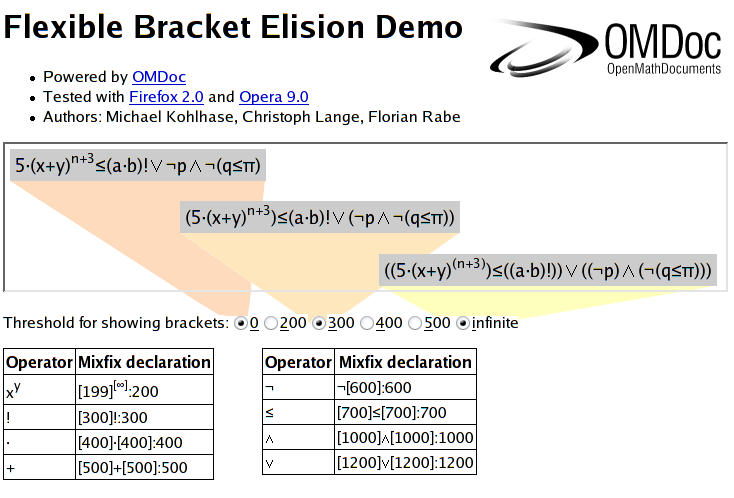
\includegraphics[width=\columnwidth]{demo-shot}
    \caption{Flexible Elision of Brackets in XHTML}
    \label{fig:flexible-elision}
\end{figure}

  We have implemented a prototypical flexible elision scheme for dynamic XHTML, by
  generating tokens for all elidable parts, wrapping them in
  {\element[ns-elt=xhtml]{span}} elements and exporting the elision group and level
  information as XML attributes {\attributeshort[ns-attr=omdoc]{egroup}} and
  {\attributeshort[ns-attr=omdoc]{elevel}} on these elements. All
  {\element[ns-elt=xhtml]{span}} elements with visibility group $g$ and level $l>T_g$ are
  augmented with the attribute {\snippet{style="display:none"}}, which elides them. If the
  user changes the threshold, an embedded {\javascript} function can be used to set the
  display property accordingly. In Figure~\ref{fig:flexible-elision}, we show the system
  with three levels of bracketing thresholds. The same technique would work for
  XHTML+MathML, if the CSS {\tt{display}} directive were implemented for {\mathml}
  elements across browsers. 
\end{newpart}

\section{The Flexary Mixfix Model in {\omdocv{1.8}}}\label{sec:preselem}

We introduce extensions making the declarative {\omdoc} syntax of presentations more
expressive. Thus we can drop the support for embedded XPath and XSLT expressions, which
represented big hurdles for implementations. 

\subsection{An XML Encoding for Flexary Mixfix Declarations}

The presentation of mathematical objects is specified by {\element{presentation}} elements
as follows:

\begin{center}\small
\begin{tabular}{|l|p{1.1cm}|p{1.1cm}|l|}\hline
  Element  &  \multicolumn{2}{c|}{Attributes}  &  Content \\\cline{2-3}
  & Required & Optional & \\\hline\hline
  presentation  & for, role,\newline format & prec.        & \llquote{item}* \\\hline
  map           & begin, end        & \llquote{e}    & separator? \llquote{item}* \\\hline
  arg           & pos      & \llquote{e}             & EMPTY\\\hline
  separator     &          & \llquote{e}             & \llquote{item}* \\\hline
  recurse       &          & \llquote{e},\newline prec. & EMPTY \\\hline
  attribution   & cd, name & \llquote{e},\newline cdbase     & \llquote{item}* \\\hline
  text          & value    & crossref                   & \#PCDATA \\\hline
  element       & name     & ns, \llquote{e},\newline crossref   & attribute* \llquote{item}*\\\hline
  attribute     & name     & ns                         & \llquote{item}* \\\hline
  name          &          &                            & EMPTY\\\hline 
  \multicolumn{4}{|p{\columnwidth}|}{\llquote{item} $\hat=$ (text $|$ element $|$ map $|$ attribution $|$
recurse)\newline
\llquote{e} $\hat=$ egroup, elevel\newline
prec. $\hat=$ precedence}\\\hline
\end{tabular}
\end{center}

The attributes of {\element{presentation}} elements have the following meaning:
\begin{itemize}
\item {\attribute{for}{presentation}}: a URI reference to a symbol to which the
  presentation applies, or to the theory for which a default presentation is given.
\item {\attribute{role}{presentation}}: the role of the presented symbol to which the
  presentation applies. The same symbol can be used in different roles\footnote{Do not
    confuse the symbols' role in the notational context specified in the
    {\attribute{role}{presentation}} attribute here with the role of a symbol in the
    {\openmath}2 standard}, and for each role a different presentation may be necessary.
  Possible values are {\attval{binder}{role}{presentation}},
  {\attval{application}{role}{presentation}}, {\attval{constant}{role}{presentation}},
  {\attval{variable}{role}{presentation}}, {\attval{key}{role}{presentation}}, and
  {\attval{error}{role}{presentation}}, mirroring the possible values of the corresponding
  attribute of the presented symbol (cf.~\cite[chapter~15.2.1]{Kohlhase:omdoc1.2}).
\item {\attribute{format}{presentation}}: A whitespace-separated list of target formats
  for which the presentation element can be used. Typical values are
  {\attval{ascii}{role}{presentation}}, {\attval{html}{role}{presentation}},
  {\attval{pmathml}{role}{presentation}}, {\attval{latex}{role}{presentation}}, and
  {\attval{default}{role}{presentation}}. The latter acts as a backup that can be applied
  if there is no specific {\element{presentation}} element for a given format.
  % \item {\attribute[ns-attr=xml]{id}{presentation}} (\cite{W3C05:xmlid}): an optional
  %   identifier that can be used to refer to a presentation, e.g., to select between
  %   alternative presentations depending on the presentation context.
\item {\attribute{precedence}{presentation}}: the output precedence of the term, which is
  used for bracket elimination. It must be an integer, or the string ``infinity'', and
  defaults to $0$.\ednote{IMHO reicht $[0,\infty)$; $(-\infty,+\infty)$ braucht man nicht.
    --CL}
\end{itemize} 
The exact syntax of the children of the {\element{presentation}} elements is introduced
when we specify their presentation behavior. The two optional attributes
{\attributeshort{egroup}} and {\attributeshort{elevel}}, which may occur on almost all
elements that relate to presentation are used to specify the elision group and elision
level. If {\attributeshort{egroup}} is omitted, it defaults to the home theory that the
containing {\element{presentation}} element applies to.

\subsection{Determining Notation Definitions}\label{sec:determining}

An application that displays a mathematical object $O$ must process $O$ recursively
looking up the needed {\element{presentation}} element once in the beginning and then
whenever a {\element{recurse}} element is encountered. This lookup is guided by the
attributes {\attribute{for}{presentation}}, {\attribute{role}{presentation}}, and
{\attribute{format}{presentation}}, which determine when a {\element{presentation}}
element is eligible. If these attributes uniquely determines a {\element{presentation}}
element, it must be used by the application. Otherwise, the application is free to choose
the most appropriate one. This choice is non-trivial and is the topic of ongoing
research~\cite{KohMueMue:dfncimk07}.

More precisely, to present an object $O$, a {\element{presentation}} element is searched
as follows.
\begin{itemize}
\item If $O$ is a binding, application, or error object with a symbol as the first child,
  a presentation for this symbol with the appropriate role. If none is found or the first
  child is not a symbol, a presentation for the home theory of $O$ with the appropriate
  role. \begin{newpart}{@FR/CL is this reasonable?\\
      @FR, you said something about making the meta-theory {\omdoc} the default. --CL}If
    this does not exist either, the presentation system falls back first to a
    format-specific-, and then a general default presentation defined by the
    system.\end{newpart}
\item If $O$ is an attributed object, a presentation for the key of the first attribution
  with role {\attval{key}{role}{presentation}}. If none is found, a presentation for the
  home theory of $O$ with that role.
\item If $O$ is a symbol, a presentation for $O$ with role
  {\attval{constant}{role}{presentation}}. If none is found, a presentation for the home
  theory of $O$ with that role.
\item If $O$ is a variable, a presentation for it that is attributed to it in its binder
  as specified in {\omdocv{1.2}}. If none is found, a presentation for the home theory of
  the binder with role {\attval{variable}{role}{presentation}}.
\item The presentation of constants and foreign objects must be determined independently
  by the application.
\end{itemize}
Of course, in all these cases only {\element{presentation}} elements with the intended
target format are eligible.

\subsection{Generating Presentations for {\openmath} Objects}

Once a {\element{presentation}} element, say with a body $B$, has been chosen for $O$, the
presentation is obtained as a function of $O$ and $B$. We say that $B$ is rendered in
context $O$.

\begin{newpart}{@FR/CL, please check\\
  OK, but we also want <arg pos="0"/> to access the operator itself. --CL}
Let $n$ be the number of components of $O$. If $n>0$ let $i$ be the value of the required
attribute {\attribute{pos}{arg}} and $p$ is the value of the (optional) attribute
{\attribute{precedence}{arg}}. Furthermore, let $\pi_n(x)\colon=x\;mod\;n$, if $x\in
[-(n-1);n-1]$, and $\pi_n(x)=x$ else. Then {\snippet{arg}} recursively calls the
presenation procedure with precedence $p$ on the $\pi_n(i)$th argument (the $\pi_n(i+1)$
component) of $O$. Note that $\pi_n(i)\in [0,\ldots,n-1]$; this allows for conveniently
accessing, e.\,g., the last component by the index $-1$, and the operator symbol by the
index $0$.

For example the presentation of a typing judgment $\Gamma\vdash_\Sigma t:T$ in {\LaTeX}
(expressing that $t$ has type $T$ in context $\Gamma$ over the signature $\Sigma$) can be
specified as follows:
\begin{lstlisting}[mathescape,label={lst:typing-judgment},
                   caption={Presenting a Typing Judgment}]
<symbol name="typing-judgment" role="application"/>
<presentation for="#typing-judgment" role="application" format="latex">
  <arg pos="1"/>
  <text>\vdash_{</text><arg pos="2"/><text>}</text>
  <arg pos="3"/>
  <text>:</text>
  <arg pos="4"/>
</presentation>
\end{lstlisting}
\end{newpart}
The only other element needed here is the {\element{text}} element, which literally
inserts its content into the output string. If the output format is XML-based the
{\element{text}} generates an XML text node.

A {\element{map}} element $M$ is interpreted as a component mapping
specification $\fimarg{\llquote{sep}:\recu{p}}{\pi_n(b)}{\pi_n(e)}$, where
\begin{enumerate}
\item $n$ is the number of children $n$ of $O$.
\item $b$ ($e$) is the value of the attribute {\attribute{begin}{map}}
  ({\attribute{end}{map}}). 
\item $p$ is the value of the {\attribute{precedence}{recurse}} attribute of the
  {\element{recurse}} element (or of the \element{presentation}) element if the the former
  is missing.
\item $\llquote{sep}$ to the result of recursively rendering the {\element{separator}}
  child of $M$ in context $O$. If there is no such child, assume $\llquote{sep}$ is the
  empty token sequence.
\end{enumerate}
If $M$ is empty, assume its content to be a child {\snippet{<recurse/>}}.

Note that {\snippet{<map begin="$n$" end="n">} \snippet{<recurse
    precedence="$p$"/></map>}} is equivalent to {\snippet{<arg pos="$n$"
    precedence="$p$"/>}}.

\begin{lstlisting}[mathescape,label={lst:multiplication},
                   caption={A Notation Definition for Multiplication}]
<symbol name="times" role="application"/>
<presentation for="#times" role="constant" format="ascii">
  <text>*</text>
</presentation>
<presentation for="#times" role="constant" format="latex">
 <text>\ast</text>
</presentation>
<presentation for="#times" role="application" format="ascii latex">
  <text egroup="lbrack">(</text>
  <map begin="1" end="-1">
    <separator><arg pos="0"/></separator>
    <recurse/>
  </map>
  <text egroup="rbrack">)</text>
</presentation>
\end{lstlisting}
Here we have used two format variants for the constant role to keep the notation
definition of the applied form as general as possible: we use {\snippet{<arg pos="0"/>}}
to call the presentation of the function symbol as a constant in the presentation of
multiplication. We rely on the recursive rendering of the arguments. Note that we have
used the {\attribute{egroup}{text}} attribute to classify the bracket characters as
such.\ednote{MK: possible inconsistency to what we said earlier, note that we could also
  use the lbrack
  and rbrack elements here, maybe?\\
  Unless we hard-code that e.g. an lbrack in PMML is ``<mo>(</mo>'' and ``('' in \TeX , I
  like @egroup better, as, depending on the output format, we need either <text> or
  <element> to generate brackets. --CL}

{\snippet{<attribution cd="\llquote{cd}" name="\llquote{name}">A</attribution>}} is
rendered by rendering $A$ in the context of the value for the key specified by the symbol
with name $\llquote{name}$ from the theory {\llquote{cd}} of the attribution of $O$. If
this attribution is not present, it is rendered as the empty string. Consider for instance
the presentation of the universal quantifier with a flexible number of possibly typed
variables:
\begin{lstlisting}[mathescape]
<symbol name="univ-quant" role="binder"/>
<presentation for="#univ-quant" role="binder" format="latex">
  <text value="\forall"/>
  <map begin="1" end="-2">
    <separator><text>,</text></separator>
    <recurse/>
    <attribution cd="types" name="type">
      <text>:</text>
      <recurse/>
    </attribution>
  </map>
  <text egroup="lbrack">.(</text>
  <arg pos="-1"/>
  <text egroup="rbrack">)</text>
</presentation>
\end{lstlisting}
Note how the bound variables appear with the indices $1$ to $-2$ and the body with index
$-1$. Also note how the colon is only printed if a type ascription is present.

\begin{newpart}{@FR: please check if this is reasonable}
  Finally, we can use the {\element{name}} element to render the value of the name
  attribute of $O$ if $O$ is a symbol or variable. For other $O$, it is not defined.
  Therefore, {\snippet{<name/>}} may only occur in a {\element{presentation}} element with
  role {\attval{constant}{role}{presentation}} or {\attval{variable}{role}{presentation}}.
  This is useful for specifying the default presentation mentioned above, for instance the
  default notation definitions
\begin{lstlisting}[mathescape]
<presentation role="constant" format="ascii">
  <name/>
</presentation>
<presentation role="variable" format="ascii">
  <name/>
</presentation>
<presentation role="applied" format="ascii" precedence="1000">
  <arg pos="0"/>
  <text egroup="lbrack">(</text>
  <map begin="1" end="-0">
    <separator><text>,</text></separator>
  </map>
  <text egroup="rbrack">)</text>
</presentation>
<presentation role="binding" format="ascii" precedence="1000">
  <arg pos="0"/>
  <text egroup="lbrack">(</text>
  <map begin="1" end="-1">
    <separator><text>,</text></separator>
  </map>
  <text egroup="rbrack">)</text>
  <arg pos="-0"/>
</presentation>
\end{lstlisting}
\end{newpart}

We have only used the ASCII-based {\LaTeX} as an example format above; for XML-based
formats, we need extra infrastructure: An {\element{element}} element is rendered as an
XML element in the obvious way. And an {\element{attribute}} element produces an attribute
of the governing XML element, the presentation of the body of the element suitably
XML-escaped yields the value of the generated attribute. For example the presentation of a
symbol that attributes a certain color in presentation {\mathml} could be given as
follows. (The value of such an attribution must be an {\element{OMFOREIGN}} element that
the application can present as text.)
\begin{lstlisting}[mathescape]
<symbol name="color" role="attribution"/>
<presentation for="#color" role="key" format="pmathml">
  <element name="mstyle">
    <attribute name="fontcolor"><arg pos="1"/></attribute>
    <arg pos="2"/>
  </element>
</presentation>
\end{lstlisting}

To get an intuition for the full power of the elision capability of the new notation
definition format, consider the following (contrived) example: assume an object $O$ with
component vector $(A_1,A_2)$ which are rendered recursively as {\snippet{<a1/>}} and
{\snippet{<a2 omdoc:egroup="group0" omdoc:elevel="0"/>}}. Then in context $O$, the
presentation
\begin{lstlisting}[mathescape]
<presentation>
  <map egroup="group1" level="1">
     <separator egroup="group2" elevel="2">
       <element name="s1" egroup="group3" elevel="3">
         <element name="s2" egroup="group4" elevel="4"/>
       </element>
     </separator>
     <recurse egroup="group5" elevel="5"/>
  </map>
</presentation>
\end{lstlisting}
is rendered as
\begin{lstlisting}[mathescape]
<a1 omdoc:egroup="group5" omdoc:elevel="5"/>
<s1 omdoc:egroup="group1" omdoc:elevel="1">
  <s2 omdoc:egroup="group4" omdoc:elevel="4"/>
</s1>
<a2 omdoc:egroup="group5" omdoc:elevel="5"/>
\end{lstlisting}
Note how the visibility information of the outermost element overrides the information of
inner elements if the outer element is a structuring element like {\element{map}},
{\element{separator,}} or {\element{recurse}}. We only mention this for the sake of
definiteness though. In practice it is unreasonable to provide so much visibility
information that it leads to such conflicts.


\paragraph{Cross-References}
In principle, the treatment of cross-references is left as in {\omdocv{1.2}}. In output
formats that are capable of cross-references, references from parts of the display to the
definition of the symbol may be generated. The {\element{presentation}} elements can
specify which parts of the presentation this reference is affixed to by using the optional
{\attributeshort{crossref}{}} attribute. This has values {\attvalshort{true}{crossref}}
and {\attvalshort{false}{crossref}}, the latter being the default. Cross-references are to
be attached to all elements for which the value is {\attvalshort{true}{role}}.

\section{Conclusion and Outlook}\label{sec:outlook}

The advantage of content-oriented representation formats for mathematical formulae is that
they are independent or a specific output format, and that human-oriented presentations
can be generated taking into account user preferences, device constraints, etc. To realize
this potential, we need presentation algorithms that are
\begin{description}
\item[knowledge-based] The knowledge about notations and their use is an integral part of
  our mathematical expertise. If a presentation algorithm is not, then it becomes
  unmaintainable.
\item[extensible] Just as mathematics itself, mathematical notation is never finished; new
  notations are always invented, and they are introduced and discarded on the fly.
\item[adaptive] They should allow to take the user's preferences into account. In the end,
  the purpose of mathematical notation is to support a reader in understanding mathematics
  as effortlessly as possible --- and people differ in their cognitive styles.
\item[mathematical] They should be able to model as many mathematical practices as
  possible, so that mathematicians are not hindered by system restrictions in the
  available notations.
\item[efficient] Presentation generation should not bog down servers, and should run on
  all kinds of clients with little lag. The time of the working mathematician is precious!
\end{description}
The first three of these aspects call for an meta-mathematical language for
{\emph{notation definitions}} which can be managed by MKM tools. A corollary of the
manageability postulate is that the notation definition language should be
{\emph{declarative}}. 

In this paper, we have presented an infrastructure for declarative notation definitions
building on ideas from {\omdocv{1.2}} and the presentation system of the {\isabelle}
theorem prover. We have incorporated functionality for flexary applications and binders
necessary to apply these ideas to {\openmath} and content {\mathml}, and we have extended
the {\isabelle}'s precedence-based elision algorithm with general flexible elision
functionality, which covers most mathematical elision practices. We conjecture that
others, like Church's dot notation can be specified by allowing more values for the
{\attributeshort{egroup}} attribute.

Actually, the dot notation is a representative of a more general, user-adaptive practice
that we do not cover in this paper: {\emph{abbreviation}}. If a formula is too large or
complex to be digested in one go, mathematicians often help their audience by abbreviating
parts, which are explained in isolation or expanded when the general picture has been
grasped. We feel that the abbreviation generation problem shares many aspects with
elisions, but is less structured, and more dependent on modeling the abilities and
cognitive load of the reader. Therefore we expect the elision techniques presented in this
paper to constitute a first step into the right direction, but also that we need more
insights to solve the abbreviation generation problem.

Another problem we have not addressed in this paper even though it is very related is the
problem of reversing generation in the parsing process for mathematical formulae\ednote{I
  guess we did in the compatibility section. --CL}: In some situations, the symbol
characteristics are sufficient to allow a mathematical software system to reconstruct the
content structure from its presentation. In the case of the {\isabelle} system, this
property is essential to ensure unambiguous input. In this paper, we will not pursue the
question of parseability, since the flexible elision of arguments is not sufficiently
understood to warrant a restriction to an invertible presentation process. In fact, we
have argued elsewhere\cite{Kohlhase04:stex} that the process of parsing mathematical
formula is AI-hard\footnote{i.e. we cannot solve the problem short of succeeding at
  Artificial Intelligence} in the worst case, since it pre-supposes a mathematical
understanding of the communicated concepts.

We have implemented the approach presented in this paper in a Scala class\ednote{@CL/FR:
  cite, is that correct?} to evaluate the expressivity and efficiency of our approach.
First results are very promising; we will release the finished implementation under an
open source license as a basis for practical presentation systems.

After a thorough evaluation we want to incorporate the presentation infrastructure
presented in this paper into the {\omdocv{1.8}} format currently under development, and we
propose it as part of the content dictionary mechanism of the upcoming {\mathml}3
recommendation.


\begin{footnotesize}
\bibliography{kwarc} 
\bibliographystyle{alpha}
\end{footnotesize}
\end{document}
%%% Local Variables: 
%%% sentence-end-double-space: nil
%%% mode: latex
%%% fill-column: 90
%%% End: 
